%% abtex2-modelo-trabalho-academico.tex, v-1.9.6 laurocesar
%% Copyright 2012-2016 by abnTeX2 group at http://www.abntex.net.br/ 
%%
%% This work may be distributed and/or modified under the
%% conditions of the LaTeX Project Public License, either version 1.3
%% of this license or (at your option) any later version.
%% The latest version of this license is in
%%   http://www.latex-project.org/lppl.txt
%% and version 1.3 or later is part of all distributions of LaTeX
%% version 2005/12/01 or later.
%%
%% This work has the LPPL maintenance status `maintained'.
%% 
%% The Current Maintainer of this work is the abnTeX2 team, led
%% by Lauro César Araujo. Further information are available on 
%% http://www.abntex.net.br/
%%
%% This work consists of the files abntex2-modelo-trabalho-academico.tex,
%% abntex2-modelo-include-comandos and abntex2-modelo-references.bib
%%

% ------------------------------------------------------------------------
% ------------------------------------------------------------------------
% abnTeX2: Modelo de Trabalho Academico (tese de doutorado, dissertacao de
% mestrado e trabalhos monograficos em geral) em conformidade com 
% ABNT NBR 14724:2011: Informacao e documentacao - Trabalhos academicos -
% Apresentacao
% ------------------------------------------------------------------------
% ------------------------------------------------------------------------

\documentclass[
	% -- opções da classe memoir --
	12pt,				% tamanho da fonte
	openright,			% capítulos começam em pág ímpar (insere página vazia caso preciso)
	oneside,			% para impressão em recto e verso. Oposto a oneside
	a4paper,			% tamanho do papel. 
	% -- opções da classe abntex2 --
	%chapter=TITLE,		% títulos de capítulos convertidos em letras maiúsculas
	%section=TITLE,		% títulos de seções convertidos em letras maiúsculas
	%subsection=TITLE,	% títulos de subseções convertidos em letras maiúsculas
	%subsubsection=TITLE,% títulos de subsubseções convertidos em letras maiúsculas
	% -- opções do pacote babel --
	english,			% idioma adicional para hifenização
	french,				% idioma adicional para hifenização
	spanish,			% idioma adicional para hifenização
	brazil				% o último idioma é o principal do documento
	]{abntex2}

% ---
% Pacotes básicos 
% ---
\usepackage{lmodern}			% Usa a fonte Latin Modern			
\usepackage[T1]{fontenc}		% Selecao de codigos de fonte.
\usepackage[utf8]{inputenc}		% Codificacao do documento (conversão automática dos acentos)
\usepackage{lastpage}			% Usado pela Ficha catalográfica
\usepackage{indentfirst}		% Indenta o primeiro parágrafo de cada seção.
\usepackage{color}				% Controle das cores
\usepackage{graphicx}			% Inclusão de gráficos
\usepackage{microtype} 			% para melhorias de justificação
% ---
		
% ---
% Pacotes adicionais, usados apenas no âmbito do Modelo Canônico do abnteX2
% ---
\usepackage{lipsum}				% para geração de dummy text
% ---

% ---
% Pacotes de citações
% ---
%\usepackage[brazilian,hyperpageref]{backref}	 % Paginas com as citações na bibl
\usepackage[alf]{abntex2cite}	% Citações padrão ABNT

% --- 
% CONFIGURAÇÕES DE PACOTES
% --- 

% ---
% Configurações do pacote backref
% Usado sem a opção hyperpageref de backref
%\renewcommand{\backrefpagesname}{Citado na(s) página(s):~}
% Texto padrão antes do número das páginas
%\renewcommand{\backref}{}
% Define os textos da citação
%\renewcommand*{\backrefalt}[4]{
%	\ifcase #1 %
%		Nenhuma citação no texto.%
%	\or
%		Citado na página #2.%
%	\else
%		Citado #1 vezes nas páginas #2.%
%	\fi}%
% ---

% ---
% Informações de dados para CAPA e FOLHA DE ROSTO
% ---
\titulo{Uma Ferramenta de Mapeamento Conceitual para Moodle integrada
	ao CMPaaS}
\autor{Israel Henrique Silva de Lima}
\local{Vitória}
\data{2016}
\orientador{Wagner de Andrade  Perin}
\coorientador{Davidson Cury}
\instituicao{
	Universidade Federal do Espírito Santo -- UFES
	\par
	Centro Tecnológico
	\par
	Departamento de Informática}
\tipotrabalho{Monografia (PG)}
% O preambulo deve conter o tipo do trabalho, o objetivo, 
% o nome da instituição e a área de concentração 
\preambulo{Monografia apresentada ao Curso de Engenharia de Computação do Departamento de Informática da Universidade Federal do Espírito Santo, como requisito parcial para obtenção do Grau de Bacharel em Engenharia de Computação.}
% ---


% ---
% Configurações de aparência do PDF final

% alterando o aspecto da cor azul
\definecolor{blue}{RGB}{41,5,195}

% informações do PDF
\makeatletter
\hypersetup{
     	%pagebackref=true,
		pdftitle={\@title}, 
		pdfauthor={\@author},
    	pdfsubject={\imprimirpreambulo},
	    pdfcreator={LaTeX with abnTeX2},
		pdfkeywords={abnt}{latex}{abntex}{abntex2}{trabalho acadêmico}, 
		colorlinks=true,       		% false: boxed links; true: colored links
    	linkcolor=blue,          	% color of internal links
    	citecolor=blue,        		% color of links to bibliography
    	filecolor=magenta,      		% color of file links
		urlcolor=blue,
		bookmarksdepth=4
}
\makeatother
% --- 

% --- 
% Espaçamentos entre linhas e parágrafos 
% --- 

% O tamanho do parágrafo é dado por:
\setlength{\parindent}{1.3cm}

% Controle do espaçamento entre um parágrafo e outro:
\setlength{\parskip}{0.2cm}  % tente também \onelineskip

% ---
% compila o indice
% ---
\makeindex
% ---

% ----
% Início do documento
% ----
\begin{document}

% Seleciona o idioma do documento (conforme pacotes do babel)
%\selectlanguage{english}
\selectlanguage{brazil}

% Retira espaço extra obsoleto entre as frases.
\frenchspacing 

% ----------------------------------------------------------
% ELEMENTOS PRÉ-TEXTUAIS
% ----------------------------------------------------------
% \pretextual

% ---
% Capa
% ---
\imprimircapa
% ---

% ---
% Folha de rosto
% (o * indica que haverá a ficha bibliográfica)
% ---
\imprimirfolhaderosto*
% ---

% ---
% Inserir a ficha bibliografica
% ---

% Isto é um exemplo de Ficha Catalográfica, ou ``Dados internacionais de
% catalogação-na-publicação''. Você pode utilizar este modelo como referência. 
% Porém, provavelmente a biblioteca da sua universidade lhe fornecerá um PDF
% com a ficha catalográfica definitiva após a defesa do trabalho. Quando estiver
% com o documento, salve-o como PDF no diretório do seu projeto e substitua todo
% o conteúdo de implementação deste arquivo pelo comando abaixo:
%
% \begin{fichacatalografica}
%     \includepdf{fig_ficha_catalografica.pdf}
% \end{fichacatalografica}

%\begin{fichacatalografica}
%	\sffamily
%	\vspace*{\fill}					% Posição vertical
%	\begin{center}					% Minipage Centralizado
%	\fbox{\begin{minipage}[c][8cm]{13.5cm}		% Largura
%	\small
%	\imprimirautor
%	%Sobrenome, Nome do autor
%	
%	\hspace{0.5cm} \imprimirtitulo  / \imprimirautor. --
%	\imprimirlocal, \imprimirdata-
%	
%	\hspace{0.5cm} \pageref{LastPage} p. : il. (algumas color.) ; 30 cm.\\
%	
%	\hspace{0.5cm} \imprimirorientadorRotulo~\imprimirorientador\\
%	
%	\hspace{0.5cm}
%	\parbox[t]{\textwidth}{\imprimirtipotrabalho~--~\imprimirinstituicao,
%	\imprimirdata.}\\
%	
%	\hspace{0.5cm}
%		1. Palavra-chave1.
%		2. Palavra-chave2.
%		2. Palavra-chave3.
%		II. Universidade Federal do Espírito Santo.
%		III. Faculdade de xxx.
%		IV. \imprimirtitulo 			
%	\end{minipage}}
%	\end{center}
%\end{fichacatalografica}
% ---



% ---
% Inserir folha de aprovação
% ---

% Isto é um exemplo de Folha de aprovação, elemento obrigatório da NBR
% 14724/2011 (seção 4.2.1.3). Você pode utilizar este modelo até a aprovação
% do trabalho. Após isso, substitua todo o conteúdo deste arquivo por uma
% imagem da página assinada pela banca com o comando abaixo:
%
% \includepdf{folhadeaprovacao_final.pdf}
%
\begin{folhadeaprovacao}

  \begin{center}
    {\ABNTEXchapterfont\large\imprimirautor}

    \vspace*{\fill}\vspace*{\fill}
    \begin{center}
      \ABNTEXchapterfont\bfseries\Large\imprimirtitulo
    \end{center}
    \vspace*{\fill}
    
    \hspace{.45\textwidth}
    \begin{minipage}{.5\textwidth}
        \imprimirpreambulo
    \end{minipage}%
    \vspace*{\fill}
   \end{center}
        
   Trabalho aprovado. \imprimirlocal, 24 de novembro de 2012:

   \assinatura{\textbf{\imprimirorientador} \\ Orientador} 
   \assinatura{\textbf{Professor} \\ Convidado 1}
   \assinatura{\textbf{Professor} \\ Convidado 2}
   %\assinatura{\textbf{Professor} \\ Convidado 3}
   %\assinatura{\textbf{Professor} \\ Convidado 4}
      
   \begin{center}
    \vspace*{0.5cm}
    {\large\imprimirlocal}
    \par
    {\large\imprimirdata}
    \vspace*{1cm}
  \end{center}
  
\end{folhadeaprovacao}
% ---

% ---
% Dedicatória
% ---
\begin{dedicatoria}
    \vspace*{\fill}
    \centering
    \noindent
    \textit{ Este trabalho é dedicado às crianças adultas que,\\
    quando pequenas, sonharam em se tornar cientistas.} \vspace*{\fill}
\end{dedicatoria}
% ---

% ---
% Agradecimentos
% ---
\begin{agradecimentos}
\end{agradecimentos}
% ---

% ---
% Epígrafe
% ---
\begin{epigrafe}
     \vspace*{\fill}
 	\begin{flushright}
 		\textit{``Não vos amoldeis às estruturas deste mundo, \\
 		mas transformai-vos pela renovação da mente, \\
 		a fim de distinguir qual é a vontade de Deus: \\
 		o que é bom, o que Lhe é agradável, o que é perfeito.\\
 		(Bíblia Sagrada, Romanos 12, 2)}
 	\end{flushright}
 \end{epigrafe}
% ---

% ---
% RESUMOS
% ---

% resumo em português
\setlength{\absparsep}{18pt} % ajusta o espaçamento dos parágrafos do resumo
\begin{resumo}
 Este trabalho apresenta o desenvolvimento de um plugin que permite a aplicação de mapas conceituais em cursos gerenciados pelo Moodle. Os mapas conceituais são uma ferramenta gráfica cuja função é a representação do conhecimento, ela pode ser aplicada no ensino de diversas formas, como por exemplo um método de avaliação de aprendizagem. O Moodle é uma plataforma amplamenta utilizada por instituições no mundo inteiro para gerenciar cursos de ensino a distância. O plugin desenvolvido neste trabalho é integrado ao CMPaaS, que trata-se de uma plataforma que integra diversas ferramentas de manipulação de mapas conceituais.

 \textbf{Palavras-chave}: Mapas Conceituais. Moodle. EaD. CMPaaS.
\end{resumo}

% resumo em inglês
\begin{resumo}[Abstract]
  \begin{otherlanguage*}{english}
    This is the english abstract.
 
    \vspace{\onelineskip}
 
    \noindent 
    \textbf{Keywords}: latex. abntex. text editoration.
  \end{otherlanguage*}
\end{resumo}


% ---
% inserir lista de ilustrações
% ---
\pdfbookmark[0]{\listfigurename}{lof}
\listoffigures*
\cleardoublepage
% ---

% ---
% inserir lista de tabelas
% ---
%\pdfbookmark[0]{\listtablename}{lot}
%\listoftables*
%\cleardoublepage
% ---

% ---
% inserir lista de abreviaturas e siglas
% ---
%\begin{siglas}
%  \item[ABNT] Associação Brasileira de Normas Técnicas
%  \item[abnTeX] ABsurdas Normas para TeX
%\end{siglas}
% ---

% ---
% inserir lista de símbolos
% ---
%\begin{simbolos}
%  \item[$ \Gamma $] Letra grega Gama
%  \item[$ \Lambda $] Lambda
%  \item[$ \zeta $] Letra grega minúscula zeta
%  \item[$ \in $] Pertence
%\end{simbolos}
% ---

% ---
% inserir o sumario
% ---
\pdfbookmark[0]{\contentsname}{toc}
\tableofcontents*
\cleardoublepage
% ---



% ----------------------------------------------------------
% ELEMENTOS TEXTUAIS
% ----------------------------------------------------------
\textual

% ----------------------------------------------------------
% Introdução (exemplo de capítulo sem numeração, mas presente no Sumário)
% ----------------------------------------------------------
\chapter{Introdução}
%\addcontentsline{toc}{chapter}{Introdução}
% ----------------------------------------------------------

\section{Objetivo}

O objetivo deste trabalho é a criar uma ferramenta que permite a utilização de mapas conceituais em cursos gerenciados pela plataforma Moodle integrado a plataforma CMPaaS.

Para alcançar o objetivo principal foram definidos os seguintes objetivos específicos:

\begin{itemize}
	\item Estudar o que são mapas conceituais e suas aplicações na educação.
	\item Estudar a arquitetura do Moodle e seus plugins.
	\item Entender a plataforma CMPaaS.
	\item Desenvolver um novo módulo para o Moodle segundo a arquiteura da plataforma e de seus plugins.   
\end{itemize} 



\section{Metodologia}

A metodologia utilizada neste projeto consiste em uma pesquisa e revisão bibliográfica sobre mapas conceituais e sua aplicação no ensino. Inclui também o estudo da arquitetura do Moodle, de forma a entender o seu funcionamento e como podem ser desenvolvidos novos módulos para adicionar novos recursos à plataforma.

O plugin desenvolvido neste trabalho será codificado em duas linguagens, JavaScript e PHP. A primeira será utilizada pois é a linguagem na qual o editor de mapas implementado no módulo utiliza. A segunda é a linguagem na qual o Moodle foi desenvolvido.  

\section{Estrutura deste trabalho}

Este trabalho será dividido nos capítulos descritos abaixo:

\begin{itemize}
	\item Capítulo 1: Apresenta a forma que o trabalho foi planejado e organizado. Este capítulo contém uma introdução sobre o projeto, seus objetivos e a metodologia de desenvolvimento.
	\item Capítulo 2: Expõe o que são mapas conceituais e a sua importância no ensino. Também conceitua educação a ditância e apresenta a plataforma Moodle.
	\item Capítulo 3: Faz uma descrição sobre a  plataforma CMPaaS e a sua arquitetura.    
	\item Capítulo 4: Descreve como foi planejado o desenvolvimento do plugin, apresentando suas funcionalidades e como será implementado.
	\item Capítulo 5: Detalha como o plugin foi desenvolvido.
	\item Capítulo 6: Apresenta o resultado final do projeto, demonstrando sua instalação, configuração e utilização.
	\item Capítulo 7: Faz uma avaliação dos resultados obtidos no trabalho e propõe trabalhos futuros.
\end{itemize} 


% ----------------------------------------------------------
% PARTE
% ----------------------------------------------------------
%\part{Preparação da pesquisa}
% ----------------------------------------------------------

% ---
% Capitulo com exemplos de comandos inseridos de arquivo externo 
% ---
% ---

% ----------------------------------------------------------
% PARTE
% ----------------------------------------------------------
%\part{Referenciais teóricos}
% ----------------------------------------------------------

% ---
% Capitulo de revisão de literatura
% ---
\chapter{Mapas conceituais e educação}\label{cap-maps}
% ---
%O que são? Quem criou? Quando surgiu? Quais os benefícios para a educação?
% ---
\section{Origem e definição de mapas conceituais}
% ---
O mapas conceituais foram criados na década de 70 durante um estudo de Novak que buscava entender como crianças aprendiam conceitos científicos \cite{Novak2005}. Durante seu estudo, Novak observou uma evolução nas proposições utilizadas pelas crianças, porém teve dificuldade de entender como esta mudança cognitiva ocorreu. Para compreender as mudanças na estruturas cognitivas observadas Novak desenvolveu um método baseado nas três ideias de Ausubel sobre a teoria da aprendizagem \cite{ausubel1963}. A primeira ideia é que novos significados são criados a partir de conceitos e proposições previamente conhecidos pelo aprendiz. A segunda, é que a estrutura cognitiva do indivíduo é organizada hierarquicamente, com conceitos mais gerais ocupando posições superiores, acima dos conceitos mais específicos e complexos. Já a terceira ideia é que durante o processo de aprendizagem os conceitos vão se tornando mais específicos e precisos.

Assim foi criada essa ferramenta gráfica, que tem como objetivo fazer uma representação do conhecimento. Um mapa conceitual é constituído por interligações entre dois ou mais conceitos através de uma palavra de forma a gerar um significado. Ele é construído ligando-se um conceito a outro, através de um arco que contém uma palavra descritiva, que é usada para criar uma relação significativa entre os conceitos. Além disso, os conceitos mais gerais estão dispostos no topo do mapa e os mais específicos na parte inferior dele. A \autoref{fig_mapconceitual} mostra um exemplo de mapa conceitual.
\begin{figure}[htb]
	\caption{\label{fig_mapconceitual}Um exemplo de mapa conceitual}
	\begin{center}
		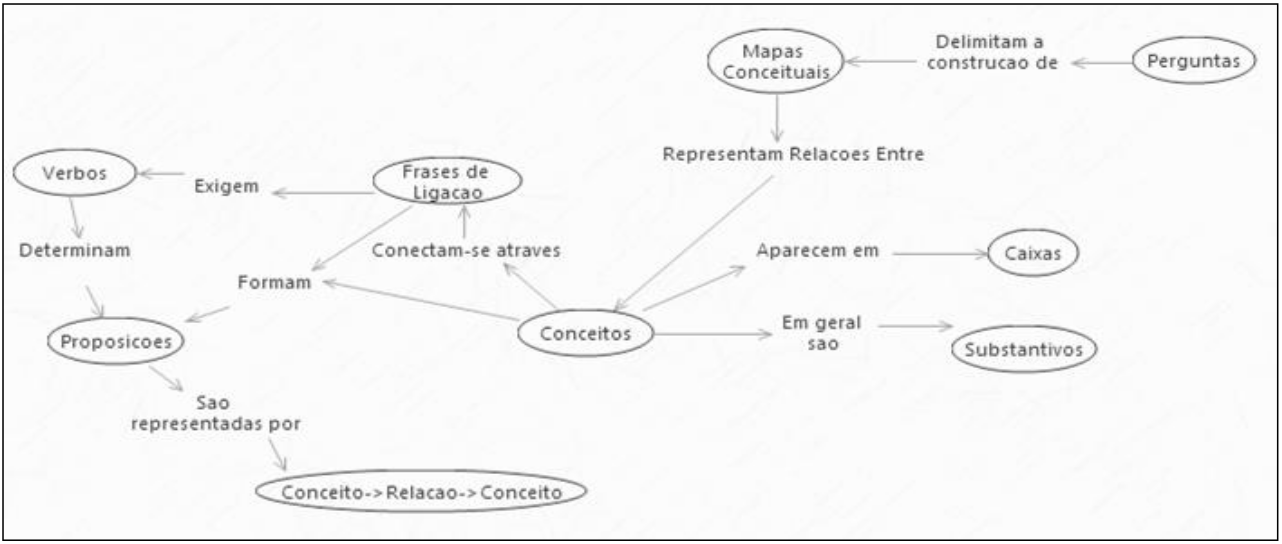
\includegraphics[scale=0.3]{mapaconceitual.png}
	\end{center}
	\legend{Fonte: \citeonline[p. 28]{Perin2014}}
\end{figure}
\section{Mapas conceituais e educação}\label{sec-mapeduc}

Os mapas conceituais podem ter diversas aplicações na educação, podem ser utilizados para representar o conhecimento adquirido em uma aula, ou então o conteúdo de um capítulo algum livro lido. Por se tratar de uma representação que é alimentada com novos conceitos conforme eles são adquiridos, pode ser utilizado pelo professor para acompanhar a aprendizagem de um estudante durante todo o período de um curso. Ademais, como os mapas conseguem representar a estrutura cognitiva de um indivíduo, eles podem ser utilizados também como método de avaliação de aprendizagem\cite{Perin2014}.

A confiabilidade da avaliação da aprendizagem tradicional,como textos dissertativos e questões de múltipla escolha, tem sido questionada por pesquisadores e educadores. Nestes tipos de teste apenas os acertos são contabilizados e os erros são descartados, isto pode fazer com que informações importantes para a avaliação sejam desprezadas.
As provas tradicionais não proporcionam a possibilidade do estudante apresentar como construiu o seu aprendizado. Elas conseguem avaliar somente a aprendizagem mecânica, não mostrando como que o aprendiz alterou suas estruturas cognitivas.
Os mapas conceituais tem se destacado como alternativa a avaliação tradicional, pois conseguem demonstrar com facilidade as modificações cognitivas que ocorrem durante o processo de aprendizagem do estudante\cite{Dutra2002}.

\section{Mapas conceituais e tecnologia da informação}

A construção de mapas conceituais é muito simples, uma caneta e um pedaço de papel são ferramentas suficientes para a confecção desse grafo. Porém a tarefa de revisá-lo, armazená-lo, e editá-lo a longo prazo  pode ser muito cansativa e complexa. A introdução do uso de computadores na confecção de mapas pode facilitar a tarefa \cite{Novak2006}.

Os primeiros programas de computadores criados com este objetivo se limitavam a mostrar apenas os mapas na tela, sem oferecer nenhum recurso adicional a ferramenta. Com a popularização do uso de computadores e da Internet houve um aumento na oferta de aplicações que tem como objetivo a construção de mapas gráficos. Porém há uma grande confusão entre usuários e desenvolvedores sobre a diferença entre mapas conceituais, organogramas e mapas mentais, devido a semelhança entre os diagramas\cite{Perin2014}. Um mapa mental, por exemplo, é muito semelhante a um mapa conceitual pois apresenta ligações entre ideias, mas ao contrario de um mapa mental não possui uma palavra descritiva ligando essas ideias e criando organicidade entre as ideias. Portanto uma aplicação de criação de mapas mentais não permite a construção de um mapa conceitual. 

Na seção 2.3 de sua dissertação de mestrado, \citeonline{Perin2014} realizou uma pesquisa sobre o estado da prática em mapas conceituais. Nela foi feito um levantamento sobre softwares que permitem a criação de mapas conceituais e quais são as funcionalidades oferecidas por eles. Nesta pesquisa foram avaliadas 16 ferramentas de edição de mapas, das quais apenas o CMapTools foi desenvolvido com o objetivo de oferecer suporte específico para mapas conceituais.

Percebendo esta carência, um grupo de pesquisadores do laboratório de Informática na Educação da Ufes propôs uma plataforma de serviços para mapas conceituais, conhecida por CMPaaS (XXXX, 2010) cujo objetivo é fornecer serviços avançados para facilitar os processos e as aplicações dos mapas conceituais, tanto no ensino quanto no mercado. Neste trabalho, interessa-nos a criação de uma ferramenta integrada ao CMPaaS que proporcione a aplicação dos mapas conceituais na Educação a Distância. 
  

%\lipsum[1]

%\lipsum[2-3]

% ----------------------------------------------------------
% PARTE
% ----------------------------------------------------------
%\part{Resultados}
% ----------------------------------------------------------

% ---
% primeiro capitulo de Resultados
% ---
%\chapter{Educação a distância}
% ---
%O que é a educação a distância?
%Qual é a origem da educação a distância?
%Qual é a importancia da educação a distância?
%Quais são as ferramentas de educação a distância?
%O Moodle
%Mapas conceituais e educação a distância.
% ---
\section{Moodle e EaD}\label{cap-ead}

Segundo \citeonline{chaves1999} EAD é um ensino que ocorre quando há uma separação física entre mestre e aprendiz, sendo utilizadas tecnologias de transmissão de voz, dados e imagens para a comunicação entre ambos. A EAD também é definida no Decreto nº 5.622 de 19 de dezembro de 2005\cite{BRASIL2005}.
 \begin{citacao}
 	Art. 1o  Para os fins deste Decreto, caracteriza-se a educação a distância como modalidade educacional na qual a mediação didático-pedagógica nos processos de ensino e aprendizagem ocorre com a utilização de meios e tecnologias de informação e comunicação, com estudantes e professores desenvolvendo atividades educativas em lugares ou tempos diversos\cite{BRASIL2005}.
 \end{citacao}
 
Em síntese é possível definir a educação a distância como um método de ensino no qual estudante e professor ficam separados fisicamente e a interação e feita através de tecnologias de comunicação (que podem ser dos mais diversos) de maneira a contornar esta separação.

Atualmente a educação a distância está relacionada ao uso de um AVA, que nada mais é que um sistema computacional cuja finalidade é prover suporte a atividades mediadas pelas tecnologias de informação e comunicação\cite{Almeida2010}. É um ambiente que tem como objetivo integrar mídias e recursos, além de apresentar informações de forma organizada e permitir interação entre estudantes, tutores e professores\cite{Franciscato2008}. Um exemplo de um AVA são os cursos que podem ser criados e gerenciados no Moodle.
   
O \begin{otherlanguage*}{english}\textit{Modular Object Oriented Distance Learning (Moodle)}\end{otherlanguage*} é sistema gerenciador de cursos que foi criado por Martin Dougiamas em 1999. Ele é uma aplicação \begin{otherlanguage*}{english}\textit{open-source}\end{otherlanguage*}, o que significa que ele é livre para ser instalado, utilizado, modificado e distribuído \cite{Dougiamas2003}. 

O \begin{otherlanguage*}{english}\textit{Moodle}\end{otherlanguage*} trabalha por padrão com cinco perfis de usuário: administrador, criador de cursos, professor, aluno e visitante. O administrador é o responsável técnico, é ele quem realiza a instalação e configuração do ambiente, além de manter ele funcionando corretamente. Já o criador de cursos tem como responsabilidade a criação e configuração dos cursos disponíveis na plataforma. Por sua vez, o professor tem como função o acompanhamento dos estudantes e a inserção de recursos e tarefas nos cursos. O aluno é quem realiza o curso, é ele quem vai utilizar os recursos e tarefas disponíveis no AVA. Por fim, o visitante é um usuário que só tem acesso as informações disponíveis na tela inicial do sistema. A \autoref{fig_moodle} mostra a interface de um curso no Moodle.


\begin{figure}[htb]
	\caption{\label{fig_moodle}Interface de um curso no Moodle}
	\begin{center}
		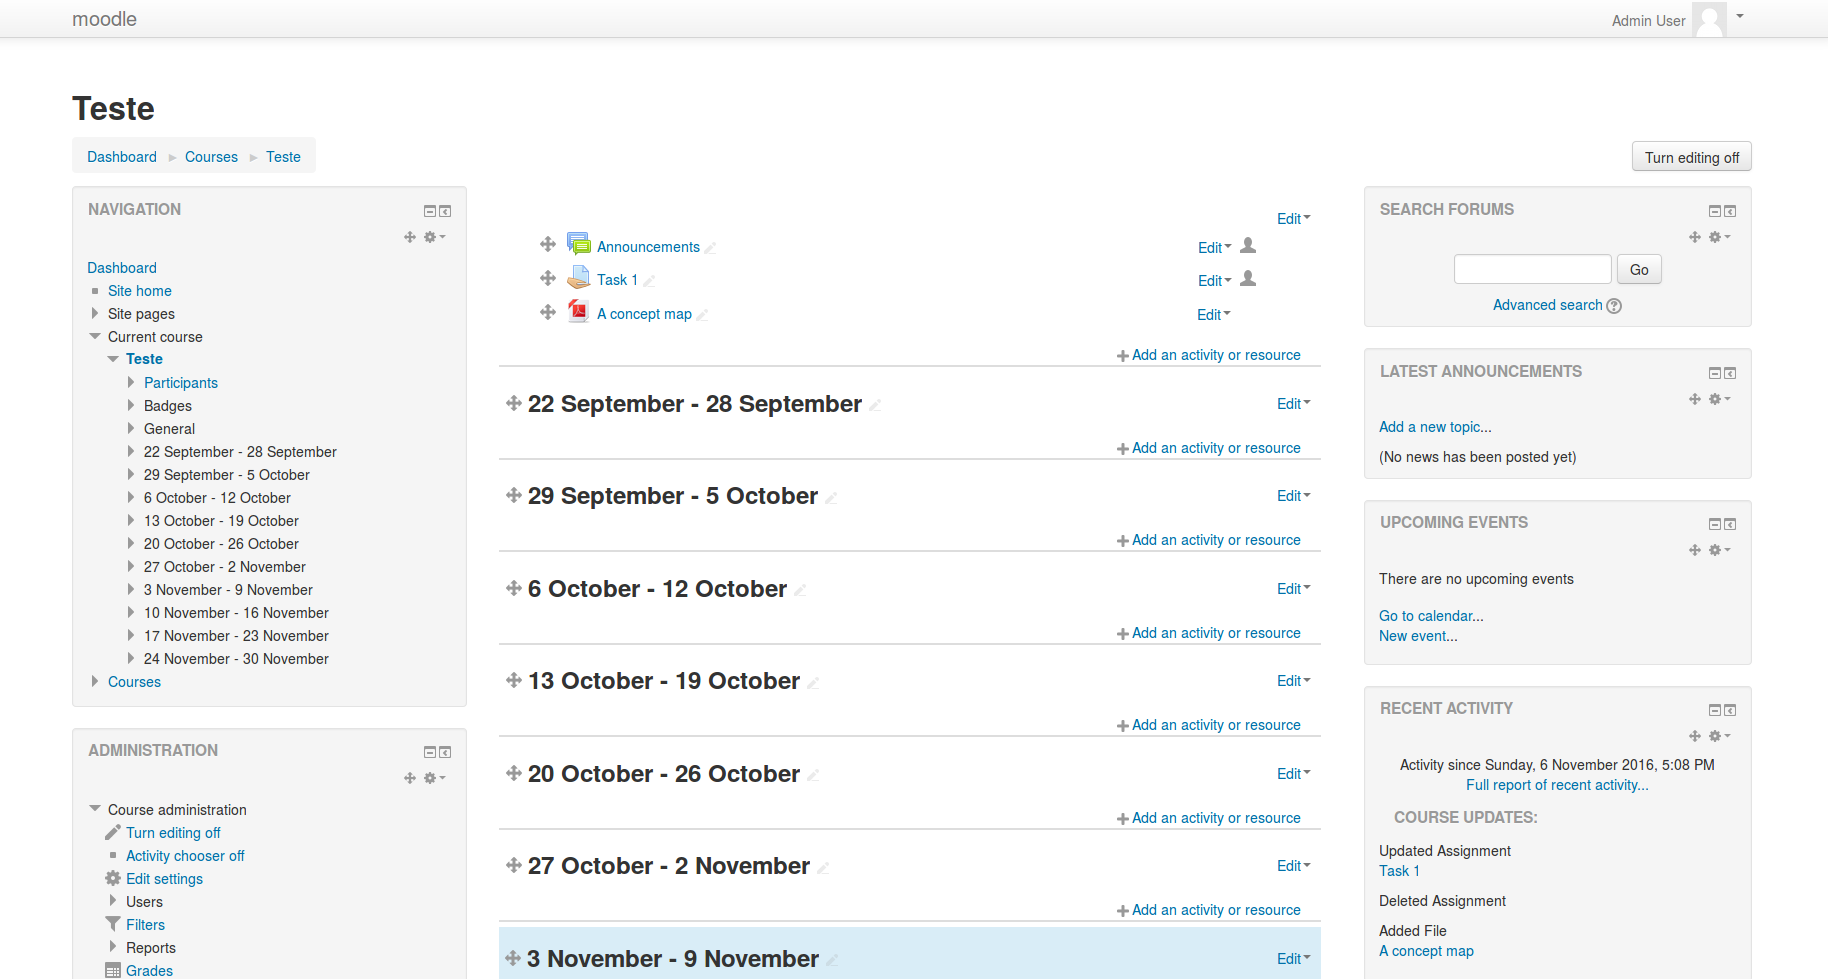
\includegraphics[scale=0.2]{moodle.png}
	\end{center}
	\legend{Fonte: Elaborada pelo autor}
\end{figure}


Ele foi escolhido para ser utilizado neste trabalho pois é amplamente usado por instituições em todo o mundo, possuindo mais de 73 mil sites registrados em 232 países\cite{MoodleStat2016}, e possui uma grande comunidade que contribui para correção de erros e criação de novas ferramentas. Além disso ele é utilizado para gerenciar os AVAs da Universidade Federal do Espírito Santo, e é muito utilizado também em diversas instituições no país, sendo o Brasil o terceiro maior utilizador da plataforma, conforme pode ser visto na \autoref{tabela-moodle}.



O fato do Moodle ser modular, ou seja, ser composto por módulos instaláveis, configuráveis e estendíveis,  permite que sejam desenvolvidos plugins e componentes que adicionam novas funcionalidades a plataforma, como é o caso do que está sendo desenvolvido neste trabalho.

O que propomos neste projeto é, portanto, a criação de um novo módulo para o Moodle que permita ao usuário construir, armazenar e recuperar seus mapas dentro desta plataforma. Além disto, propomos uma arquitetura para integração do Moodle com o CMPaaS de modo a permitir que mapas produzidos dentro da Plataforma Moodle sejam sincronizados com a Nuvem oferecida pelo projeto CMPaaS. No capítulo a seguir será possível conhecer as características básicas do CMPaaS e os serviços oferecidos por esta plataforma.

\begin{table}[htb]
	\IBGEtab{%
		\caption{Os 10 países que mais utilizam o Moodle.}%
		\label{tabela-moodle}
	}{%
	\begin{tabular}{ccc}
		\toprule
		País & Sites Registrados \\
		\midrule \midrule
		Estados Unidos & 10.131 \\
		\midrule 
		Espanha & 7.067 \\
		\midrule 
		Brasil & 4.401 \\
		\midrule 
		Reino Unido & 3.486 \\
		\midrule 
		México & 3.464 \\
		\midrule 
		Alemanha & 2.444 \\
		\midrule 
		Itália & 2.414 \\
		\midrule 
		Austrália & 2.324 \\
		\midrule 
		Colômbia & 2.264 \\
		\midrule 
		Rússia & 1.993 \\
		\bottomrule
	\end{tabular}%
}{%
\fonte{\citeonline{MoodleStat2016}}%
}
\end{table}

% ---}


% ---
% segundo capitulo de Resultados
% ---

% ---
%O que é o CMPAAS?
%Quando foi criado?
%Porque foi criado? Qual é a sua importância?
% ---
\chapter{CMPAAS}
\section{Origem}

Na \autoref{sec-mapeduc} vimos como os mapas conceituais são importantes para educação, seja para auxiliar o estudante a aprender novos conceitos, ou como método de avaliação, além de algumas outras aplicações educacionais. 

Apesar de haver este grande interesse acadêmico em ferramentas computacionais para criação e manipulação de mapas, a fragmentação das pesquisas nesta área impede que o desenvolvimento destas aplicações ocorra de forma acelerada. Assim, a integração de ferramentas já existentes facilitaria o progresso de novas pesquisas.

Se houvesse uma infraestrutura de apoio a criação e manipulação de mapas conceituais o desenvolvimento de novas ferramentas seria facilitado. Um pesquisador poderia criar uma nova solução mais facilmente se não houvesse a necessidade dele se preocupar com toda uma estrutura de gestão de mapas. Por exemplo, alguém que queira desenvolver uma aplicação que avalie mapas conceituais poderia utilizar o conteúdo existente previamente em uma solução computacional de criação e armazenamento de mapas.

Um outro problema apontado por \citeonline{Perin2014} é a dificuldade que a sociedade tem para acessar os resultados das pesquisas.
\begin{citacao}
	Consideramos importante a criação de um mecanismo de
	acesso eficiente aos resultados das pesquisas científicas, para que a comunidade possa contribuir para a evolução delas. O que propomos, portanto, é o lançamento de bases para uma convivência mais estreita entre o mundo acadêmico e a sociedade em geral.\cite{Perin2014}.
\end{citacao}
% ---

Assim foi proposto por \citeonline{Perin2014} a criação de uma plataforma denominada CMPaaS, cujo objetivo é possibilitar que a comunidade em geral acesse o resultado de pesquisas acadêmicas e prover uma infraestrutura que permita que esta comunidade crie e estenda suas funcionalidades.

\section{A plataforma CMaaS}

\subsection{Computação em Nuvem}

O termo computação em nuvem teve sua origem em 2006 durante uma palestra Eric Schmidt sobre como o Google gerenciava seus servidores\cite{taurion2009}. A palavra nuvem é uma abstração para a Internet e toda a sua complexidade de infraestrutura, arquiteturas e componentes. A computação em nuvem é um paradigma no qual o processamento, armazenamento e ferramentas computacionais são oferecidos como um serviço através da Internet. Aplicações baseadas nesta tecnologia possuem a característica de serem extensíveis e facilmente incorporadas a outras que precisem consumir os seus serviços\cite{Perin2014}.

A plataforma CMPaaS usa esta capacidade de expansão e integração da computação em nuvem para oferecer serviços de criação, edição e gestão de mapas conceituais que poderão ser acessados por qualquer usuário no mundo.

\subsection{Arquitetura}

O CMPaaS é uma plataforma que tem como objetivo integrar ferramentas de mapas conceituais e permitir acesso a elas pela comunidade. Ele possui uma arquitetura orientada a serviços, isto é, uma arquitetura que vai oferecer serviços que podem ser consumidos por outras aplicações. Por exemplo, um editor de mapas conceituais pode gerar um mapa que vai ser usado por uma aplicação que avalia mapas de forma automatizada.

Os serviços do CMPaaS são oferecidos através da Internet, podendo ser acessado de qualquer plataforma. Mas é necessário que exista um portal ou site associado a plataforma CMPaaS para que as ferramentas possam ser acessadas através de um navegador de Internet. Este portal foi nomeado como "Portal do Conhecimento"\cite{Perin2014}. 


\begin{figure}[htb]
	\caption{\label{fig_cmpaas}(a) Integração do Portal do Conhecimento com o CMPaaS. (b) Integração do CMPaaS com serviços externos}
	\begin{center}
		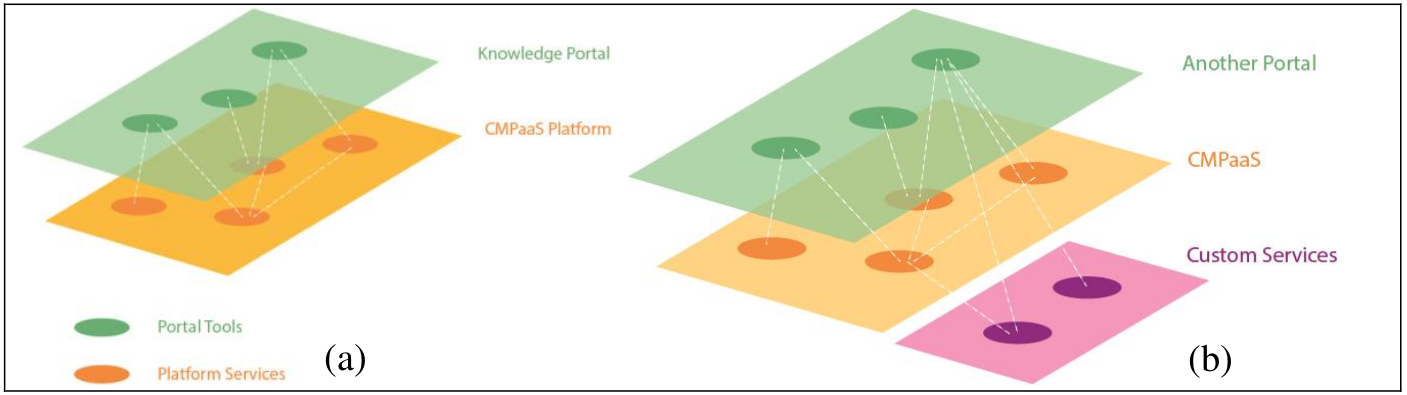
\includegraphics[scale=0.3]{cmpaas.png}
	\end{center}
	\legend{Fonte: \citeonline[p. 81]{Perin2014}}
\end{figure}

A \autoref{fig_cmpaas} ilustra a arquitetura do CMPaaS e como as aplicações fornecidas pelo portal utilizam os serviços da plataforma, muitas vezes consumindo mais de um serviço que é oferecido por ela. Além disso, é ilustrado também como um portal externo pode aproveitar os serviços disponíveis no CMPaaS, como é o caso do plugin que será apresentado posteriormente neste trabalho. Ele trata-se de um editor de mapas conceituais que armazena os mapas, criados por ele, na plataforma. Assim ele utiliza dois serviços fornecidos pelo CMPaaS, o de armazenagem de mapas e o de autenticação.

A estrutura interna da plataforma é composta por cinco camadas: serviços externos são os serviços oferecidos pelo CMPaaS aos usuários (é o que aparece no site para o usuário); processos de negócio são as rotinas que ocorrem internamente no CMPaaS; componentes internos são as aplicações internas da plataforma; serviços de aplicações externas são serviços produzidos por ferramentas externas e são consumidos por componentes do CMPaaS; e os serviços de aplicações internas são serviços produzidos por ferramentas internas do CMPaaS e são consumidos por componentes do CMPaaS.

\subsection{Serviços oferecidos}



 

\chapter{O Projeto}\label{cap-projeto}
% ---
%O que é um plugin do moodle?
%Como é feito o plugin?
%Como foi feito o plugin
% ---

\section{O problema}

Vimos no \autoref{cap-maps} que os mapas conceituais são muito importantes para a educação, principalmente como alternativa para os métodos de avaliação tradicionais. Também, no \autoref{cap-ead} foi apresentado o conceito de educação a distância e como ela é oferecida através do uso de AVAs. Sendo o Moodle apontado como um gerenciador de cursos amplamente utilizado por instituições brasileiras. Sendo assim, o suporte do Moodle para a utilização de mapas conceituais em cursos gerenciados por ele permitiria que estudantes e professores pudessem ter acesso a esta ferramenta educacional tão versátil.    

No entanto, ao buscar na lista de plugins do Moodle alguma ferramenta que permite o uso de mapas conceituais como resposta de atividades avaliativas, só foi encontrado um único plugin. Este plugin permite que questionários possam ser respondidos com uma mapa. Porém, a última atualização desta ferramenta foi no início de 2015 e ele não é compatível com as novas versões da plataforma. Portanto, não há nenhuma ferramenta que permita o uso de mapas conceituais em tarefas de cursos gerenciados pela plataforma em suas versões mais recentes.


\section{A solução proposta}

Este trabalho propõe a criação de um plugin que adicione ao Moodle de resposta de uma tarefa com um mapa conceitual. Além disso, ele será integrado a plataforma CMPaaS, consumindo serviços oferecidos por ela.

\section{Arquitetura}

O Moodle é composto por vários módulos independentes, sendo cada um deles responsável por uma funcionalidade que a plataforma oferece. O escopo deste trabalho é o desenvolvimento de um novo módulo. O plugin que foi criado neste trabalho é do tipo assignment submission plugin, ou seja, é um módulo de submissão de tarefa. O módulo de tarefa permite que um professor crie uma atividade, avaliativa ou não, para os estudantes realizarem.

Este tipo de plugin é divido em três partes:
\begin{itemize}
	\item configurações, que são opções de comportamento do módulo.
	\item sumário de envio, que será visto pelo estudante e avaliadores na tela inicial da tarefa.
	\item formulário de envio, que é onde o estudante responde a tarefa.  
\end{itemize} 

%O plugin desenvolvido neste trabalho permite que o estudante crie um mapa conceitual, modifique sua aparência e envie para avaliação. O estudante poderá também editar um mapa que já foi enviado, além de ter a possibilidade de salva-lo na plataforma CMPaaS. A \autoref{fig_casosuso} apresenta os casos de uso do plugin.
%
Este plugin oferece as seguintes funcionalidades:

\begin{itemize}
	\item criação de um novo mapa conceitual utilizando um editor de mapas. Esta funcionalidade é representada pelo caso de uso Criar Mapa.
	\item armazenagem do mapa criado no banco de dados do Moodle. Esta funcionalidade é representada pelo caso de uso Salvar Mapa.
	\item edição de um mapa previamente salvo no banco de dados do Moodle. Esta funcionalidade é representada pelo caso de uso Salvar Mapa.
	\item alteração da aparência de uma mapa que está sendo criado ou modificado no editor. Esta funcionalidade é representada pelo caso de uso Formatar Mapa.  
	\item possibilidade de salvar o mapa que está sendo criado na plataforma CMPaaS. Esta funcionalidade é representada pelo caso de uso Salvar Mapa no CMPaaS.  
	\item visualizar um mapa salvo para que possa ser avaliado. Esta funcionalidade é representada pelo caso de uso Visualizar Mapa.    
\end{itemize} 

\begin{figure}[!h]
	\caption{\label{fig_casosuso} Casos de Uso}
	\begin{center}
		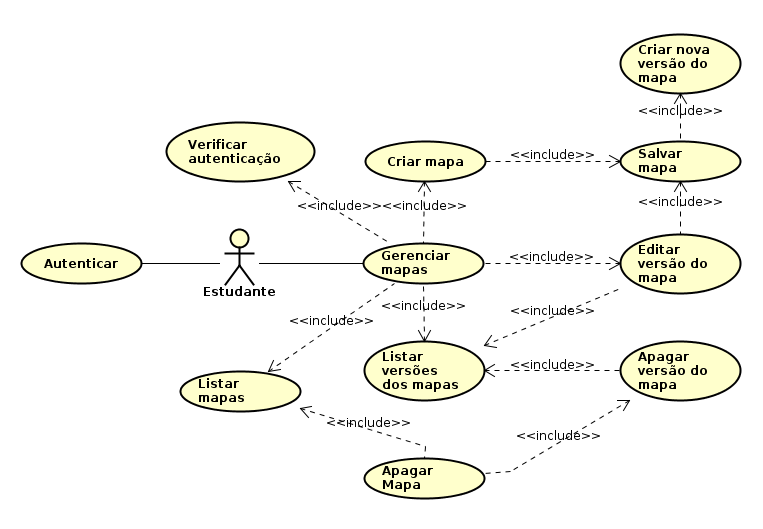
\includegraphics[scale=0.7]{casosuso.png}
	\end{center}
	\legend{Fonte: Elaborado pelo autor}
\end{figure} 

Os atores que irão utilizar o plugin são o Estudante, que irá criar e editar mapas conceituais que serão submetidos a avaliação, e um Avaliador, que irá visualizar os mapas criados pelos estudantes e avalia-los. Os atores e casos de uso são representados na \autoref{fig_casosuso}.

O caso de uso Salvar Mapa é apresentado na \autoref{fig_seq1}. Quando o estudante solicita que o mapa seja salvo a interface do plugin chama a rotina da API do Moodle responsável por enviar os dados do formulário para serem armazenados. Após esta rotina ser executada e o mapa ser armazenado um sumário do envio é apresentado ao estudante.

\begin{figure}[htb]
	\caption{\label{fig_seq1} Diagrama de Sequencia do Caso de Uso Salvar Mapa}
	\begin{center}
		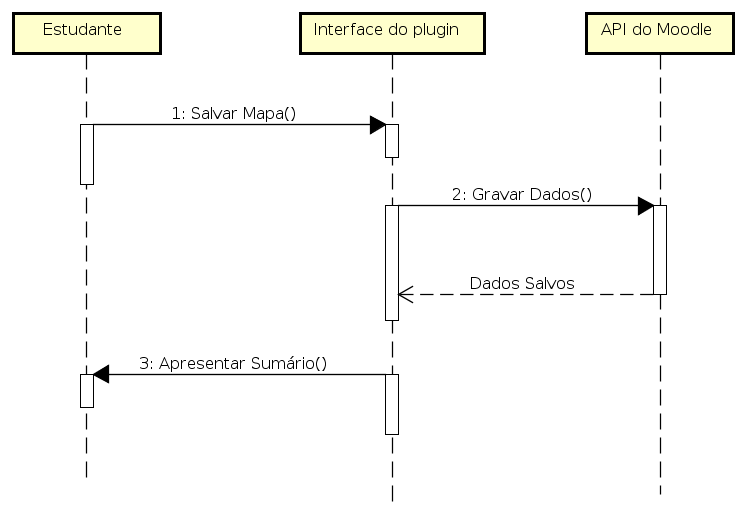
\includegraphics[scale=0.5]{SeqDiagramPlugin.png}
	\end{center}
	\legend{Fonte: Elaborado pelo autor}
\end{figure} 

\begin{figure}[htb]
	\caption{\label{fig_seq2} Diagrama de Sequencia do Caso de Uso Sincronizar Mapa}
	\begin{center}
		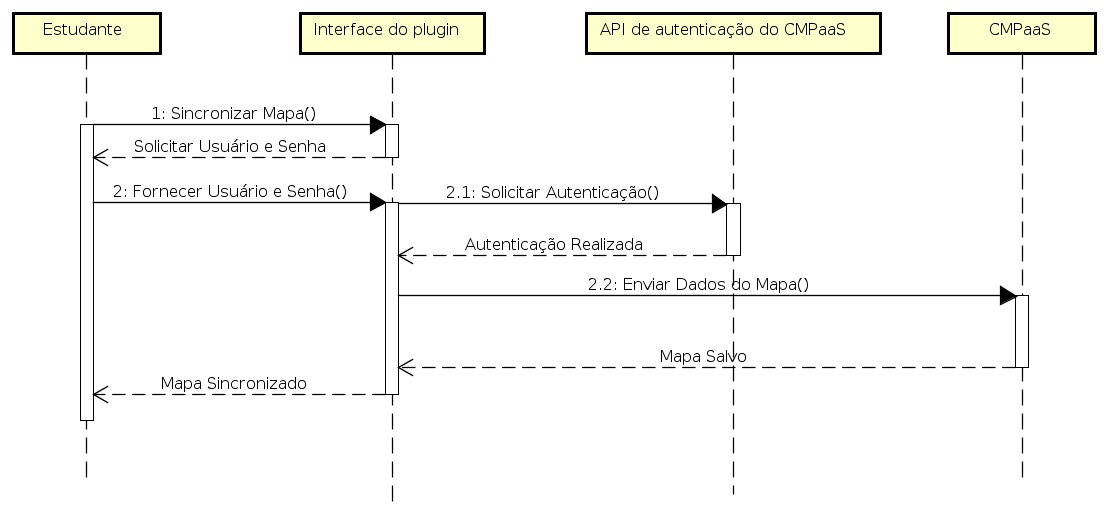
\includegraphics[scale=0.5]{SeqDiagramCmpaas.png}
	\end{center}
	\legend{Fonte: Elaborado pelo autor}
\end{figure} 

O caso de uso Sincronizar Mapa é apresentado na \autoref{fig_seq2}. É este caso de uso que realiza a integração do plugin com a plataforma CMPaaS. Quando o estudante executa a ação de sincronização do mapa a interface do plugin chama uma rotina para que seja feita autenticação no portal. Depois que o estudante é autenticado no CMPaaS os dados do mapa são enviados para serem armazenados na plataforma.

\section{Tecnologias utilizadas}

\subsection{JavaScript}

O JavaScript é uma linguagem orientada a objeto criada em 1995 por Brendan Eich que foi idealizada para permitir que pessoas que não são programadoras pudessem estender as funcionalidades de sites de Internet\cite{Richards2010}. Ela é uma linguagem interpretada, e apesar de ter sido criada para desenvolvimento web, ela é uma linguagem de proposito geral, e pode ser usada para o desenvolvimento de qualquer tipo de aplicação\cite{flanagan2006}.

Ela foi escolhida para ser utilizada neste projeto pois o editor de mapas disponível no CMPaaS foi desenvolvido com esta tecnologia e, além disso, trata-se de uma linguagem compatível com todos os navegadores modernos.  

\subsection{Json}

O JavaScript Object Notation (Json) é uma linguagem em formato de texto cuja função é a serialização de dados estruturados. A serialização é o processo de transformar objetos em um fluxo de bytes para ser armazenado em um banco de dados ou disco. Ele pode ser utilizado para representar tipos primitivos, como cadeia de caracteres e números, ou tipos estruturados, como objetos e vetores\cite{crockford2006}. Ele é utilizado para intercambio de dados entre os serviços da plataforma CMPaaS.  

\subsection{PHP}
% ---
PHP é um acrônimo recursivo para PHP: Hypertext Preprocessor, originalmente ele foi criado como uma linguagem de script estruturada cuja finalidade era o desenvolvimento de aplicações com a funcionalidade de geração de HTML dinâmico. Com o passar do tempo a linguagem evoluiu e passou a oferecer recursos para o desenvolvimento orientado a objeto\cite{minetto2007}.

A plataforma Moodle e seus plugins são desenvolvidos em PHP, por isto esta linguagem foi utilizada neste projeto. 

\chapter{Desenvolvimento}

\section{Serviço de Edição de Mapas}
O serviço de edição de mapas foi implementado com a utilização do editor de mapas conceituais disponível no CMPaaS. Ele foi desenvolvido utilizando GoJS, que é uma biblioteca em JavaScript para criação de diagramas para navegadores de Internet.

Este editor foi desenvolvido de forma a salvar os mapas no formato Json, de forma a facilitar que outras aplicações utilizem os dados que ele produz. Ele foi feito desta forma devido a proposta do CMPaaS de permitir a interoperabilidade dos serviços oferecidos.

A primeira parte do trabalho foi realizar um aprimoramento deste editor, adicionando funções para a formatação dos mapas criados por ele. Inicialmente não existia a possibilidade de alterar a fonte da letra dos conceitos ou a cor de fundo dos nós. Uma barra de ferramenta foi adicionada ao editor original para que funções de formatação estivessem disponíveis.

\begin{figure}[htb]
	\caption{\label{fig_barraformacao} Editor com barra de formatação}
	\begin{center}
		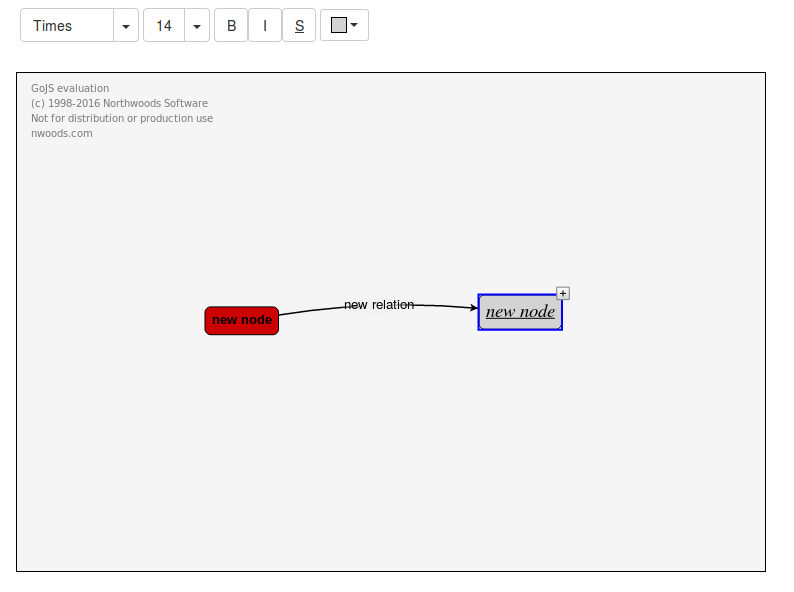
\includegraphics[scale=0.5]{barraformacao.png}
	\end{center}
	\legend{Fonte: Elaborada pelo autor}
\end{figure}

% ---
\subsection{Implementação das funções de formatação}
O editor de mapas é dividido em dois componentes, um Model e um Diagram. O Model é o que contém os dados do mapa que está sendo criado, nele os nós e links são descritos por vetores de objetos JavaScript. Já o Diagram é usado para visualizar os dados contidos no modelo.

Na \autoref{fig_gojs} temos um trecho de código que gera um diagrama simples em GoJS. Nele é criado um Model que possui um vetor com três objetos JavaScripts, nomeados Alpha, Beta e Gamma. Este vetor de objetos da classe Node representa três nós que serão apresentados no diagrama. O Model nomeado myModel é então adicionado ao Diagram chamado myDiagram. Este trecho de código gera o diagrama ilustrado na \autoref{fig_diagram}.

\begin{figure}[htb]
	\caption{\label{fig_gojs} Componentes do GoJS}
	\begin{center}
		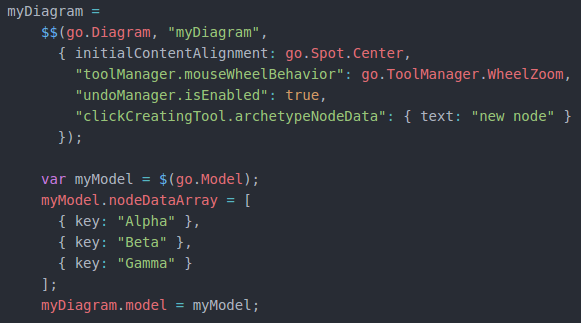
\includegraphics[scale=0.7]{gojs.png}
	\end{center}
	\legend{Fonte: Elaborada pelo autor}
\end{figure}

\begin{figure}[htb]
	\caption{\label{fig_diagram} Um diagrama gerado em GoJS}
	\begin{center}
		
\includegraphics[scale=0.7]{diagram.png}
	\end{center}
	\legend{Fonte: Elaborada pelo autor}
\end{figure}

Cada nó do mapa criado pelo editor é representado por um objeto da classe Node, que por sua vez, é composto por blocos que determinam a sua aparência. Os blocos que o editor utiliza são o Shape e o TextBlock. A classe Shape é utilizada para mostrar uma forma geométrica colorida. Já a classe TextBlock tem como função mostrar um texto. Ambas as classes possuem diversas propriedades que servem para determinar a sua aparência e o seu comportamento no diagrama.

Os trechos de código abaixo são usados para criar um Shape e um TextBlock. A forma geométrica  desenhada é retângulo com largura de 40 pixels, altura de 60 pixels, com margem de 4 pixels e preenchimento na cor vermelha. Já o TextBlock criado é um texto “a Text Block” de cor vermelha.

\begin{figure}[htb]
	\caption{\label{fig_gojselements} Código dos elementos Shape e TextBlock}
	\begin{center}
		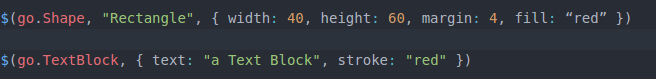
\includegraphics[scale=0.6]{gojselements.png}
	\end{center}
	\legend{Fonte: Elaborada pelo autor}
\end{figure}

As novas funcionalidades de formatação adicionadas ao editor modificam as propriedades dos objetos das classes Shape e TextBlock, alterando assim a aparência deles. Foram criados seis botões de formatação com as funções de alterar o tipo de fonte, aumentar o tamanho da fonte, alterar o estilo do texto para negrito, itálico e sublinhado, e para alterar a cor de preenchimento dos nós. Os botões de formatação de fonte alteram a propriedade font da TextBlock, que deve ser uma string  CSS. Já o botão que altera a cor do nó modifica a propriedade fill da Shape.

As funcionalidades de formatação foram implementadas em JavaScript no arquivo toolbar.js. Elas foram desenvolvidas de forma semelhante, utilizando eventos disparados pelos botões da barra de ferramenta.

Para realizar alteração de estilo da fonte e de cor do nó foram implementadas funções que modificam os atributos dos nós. Para cada botão da barra de ferramenta foi criada uma rotina que aguardava um evento disparado por ele. Quando ele ocorre uma função é chamada e realiza a modificação referente ao botão que foi acionado. 

A \autoref{fig_listener} mostra a rotina que altera a cor de preenchimento de um nó. Inicialmente é criada uma espera para o evento que será disparado pelo botão, no caso o evento input. Quando ele ocorre é chamada a função que altera a propriedade fill do objeto Shape de todos os nós selecionados, mudando assim a cor dos mesmos. As funcionalidades de estilo da fonte são implementadas com a mesma rotina, o que muda é a propriedade alterada, que passa a ser a font do objeto TextBlock de todos os nós selecionados.    

\begin{figure}[htb]
	\caption{\label{fig_listener} Rotina que altera a cor de preenchimento de um nó}
	\begin{center}
		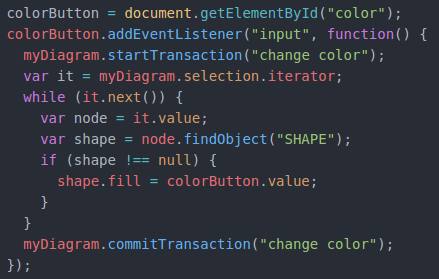
\includegraphics[scale=0.6]{listener.png}
	\end{center}
	\legend{Fonte: Elaborada pelo autor}
\end{figure}




\section{Implementação no Moodle} 
Para implementar o serviço de edição de mapas no Moodle foi utilizado um plugin já existente na plataforma como modelo. Conforme visto no \autoref{cap-projeto} o módulo escolhido para a implementação da funcionalidade de edição de mapas foi o de envio de tarefa. Todos os plugins deste tipo possuem uma estrutura de arquivo padrão, que será detalhada abaixo.
\begin{itemize}
	\item version.php: este arquivo contém informações sobre a versão do plugin, é utilizado para que o Moodle instale e atualize o plugin corretamente.
	\item settings.php: este arquivo permite que se adicione opções personalizadas para a página configuração do plugin.
	\item lang/en/submission\_nomedoplugin.php:  este é o arquivo de linguagem, ele é usado para internacionalização do plugin.
	\item db/access.php: e utilizada para adicionar capacidades adicionais ao plugin. Este arquivo é opcional, não sendo necessário se o plugin não tiver capacidades adicionais.
	\item db/upgrade.php: este arquivo define a rotina de atualização do plugin. 
	\item db/install.xml: este arquivo define as tabelas de banco de dados que o plugin vai utilizar. 
	\item db/install.php: contem o código de instalação do plugin.
	\item db/locallib.php: é o arquivo mais importante, é ele que define todas as funcionalidades do plugin.    
\end{itemize} 

\subsection{Desenvolvimento do plugin}
O plugin utilizado como base para o desenvolvimento deste trabalho foi o de envio de texto online, nele o estudante tem a possibilidade responder uma tarefa por meio de um texto escrito diretamente na plataforma. Este projeto foi desenvolvido aplicando engenharia reversa a este plugin, buscando entender a sua funcionalidade e assim descobrir como modificá-lo para transformá-lo em um editor de mapas.

O módulo de envio de texto online pode ser dividido em duas partes, uma é o editor de textos onde o estudante realiza a sua tarefa e a outra e o sumário da atividade onde tanto o estudante quanto o avaliador tem acesso ao conteúdo da tarefa enviada. O módulo desenvolvido neste trabalho mantém esta estrutura, alterando o editor de textos por um de mapas conceituais e alterando o sumário de forma que o conteúdo apresentado nele passa a ser um json do mapa invés de um texto.

As alterações feitas no plugin de envio de texto online se concentraram no arquivo locallib.php, que é o que determina o comportamento e funcionalidades do módulo. Dentro deste arquivo, as mudanças ocorreram nas funções get\_form\_elements(), que constrói o formulário de envio de tarefa, e no arquivo save(), que realiza a submissão do conteúdo criado pelo estudante.

A primeira parte do trabalho foi substituir o formulário de envio de texto pelo editor de mapas conceituais. Esta modificação foi realizada na função get\_form\_elements(). O código que realizava a inserção do editor de texto foi substituído por um outro, que insere um iframe contendo o editor de mapas do CMPaaS. 

Feito isto, o plugin já apresentava o editor de mapas, porém ainda era necessário salvar o mapa criado no banco de dados do Moodle. Para realizar isto o json do editor contido no iframe precisava ser salvo em algum campo de formulário. Para solucionar isto, foi criado um entrada de dados, oculta na página da tarefa, responsável por receber o json do mapa criado no editor.

Assim, quando o estudante aciona o botão de submissão da tarefa, o json do mapa que ele criou e salvo em um campo de formulário e então armazenado no banco de dados do Moodle.

Para finalizar, foi necessário criar uma forma de o editor de mapas carregar o mapa salvo pelo estudante, para caso ele tivesse interesse em editar um mapa já armazenado. A solução para isto foi realizar o caminho inverso que foi feito ao salvar o mapa criado. Ao carregar o formulário de edição de mapas o json armazenado no banco de dados e carregado em um campo oculto e um código JavaScript se encarrega se obter o conteúdo dele e carregar no mapa.

Então a primeira parte do desenvolvimento do plugin foi concluída, o estudante conseguia criar um mapa no editor, salvar o seu conteúdo na plataforma e editar novamente caso fosse necessário. Porém ainda havia a necessidade de permitir que o avaliador tivesse acesso ao conteúdo gerado pelo aluno e, além disso, proposta do trabalho era a criação de um plugin integrado com o CMPaaS,  portanto a segunda parte do trabalho e realizar esta integração e criar uma forma de o avaliador visualizar o mapa.

\subsection{Integração com o CMPaaS}

A integração do plugin com o CMPaaS é feita com a utilização de dois serviços oferecidos pela plataforma. Eles são o serviço de autenticação e o de persistência de mapas.

O serviço de autenticação é responsável por autorizar o acesso do usuário do Moodle ao CMPaaS. Quando o botão de sincronização é acionado é enviado uma mensagem pedindo autorização para que o usuário do Moodle tenha acesso ao serviço de mapas da plataforma. A API de autenticação do CMPaaS então responde concedendo acesso ao usuário do plugin ao repositório de mapas.

Após a rotina de autenticação ter sido realizada o editor de mapas envia um json com os dados do diagrama a ser sincronizado. Então o serviço de mapas do CMPaaS recebe o json e realiza a persistência do mesmo em sua base de dados.



\chapter{Implementação e Testes}

\section{Como instalar}
A pasta contendo os arquivos do plugin deve ser copiada para o diretório do moodle mod/assign/submission/. Após copiar os arquivos para este local é necessário acessar o moodle com um usuário com perfil de administrador. Assim que efetuar login irá aparecer uma mensagem de instalação de plugin, conforme a \autoref{fig_installplugin}.
\begin{figure}[htb]
	\caption{\label{fig_installplugin} Configurando a tarefa para utilizar o plugin}
	\begin{center}
		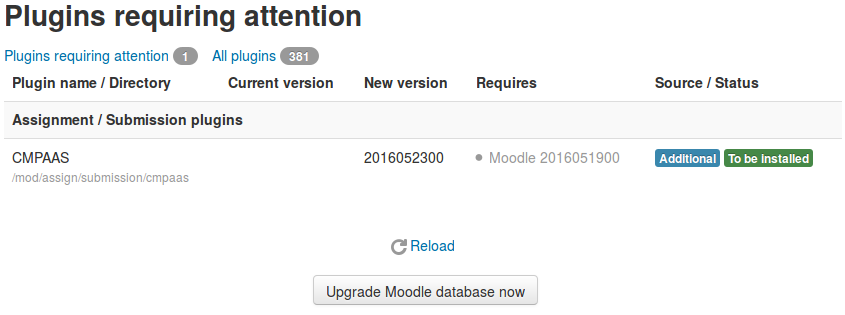
\includegraphics[scale=0.4]{installplugin.png}
	\end{center}
	\legend{Fonte: Elaborada pelo autor}
\end{figure}

Ao clicar no botão de atualização do banco de dados do Moodle o plugin será instalado e poderá ser visto na lista de plugins, conforme \autoref{fig_listaplugin}.

\begin{figure}[htb]
	\caption{\label{fig_listaplugin} Lista de plugins instalados}
	\begin{center}
		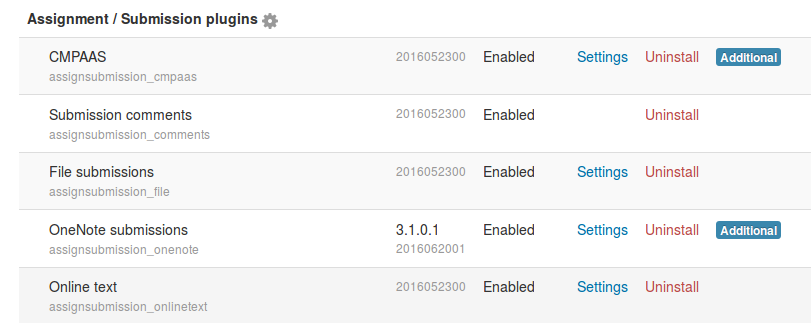
\includegraphics[scale=0.4]{listaplugin.png}
	\end{center}
	\legend{Fonte: Elaborada pelo autor}
\end{figure}

Depois do plugin ser instalado é necessário realizar a configuração da tarefa para utiliza-lo. Para que a tarefa utilize o plugin para submissão de dados é necessário selecioná-lo na tela de configuração da atividade, conforme ilustrado na \autoref{fig_configplugin}.

\begin{figure}[htb]
	\caption{\label{fig_configplugin} Configurando a tarefa para utilizar o plugin}
	\begin{center}
		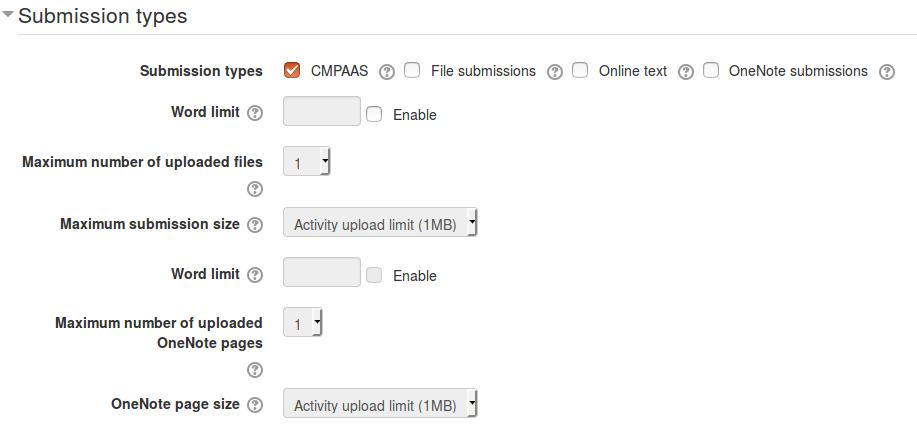
\includegraphics[scale=0.4]{configplugin.png}
	\end{center}
	\legend{Fonte: Elaborada pelo autor}
\end{figure}

\begin{figure}[htb]
	\caption{\label{fig_editor} Editor de mapas}
	\begin{center}
		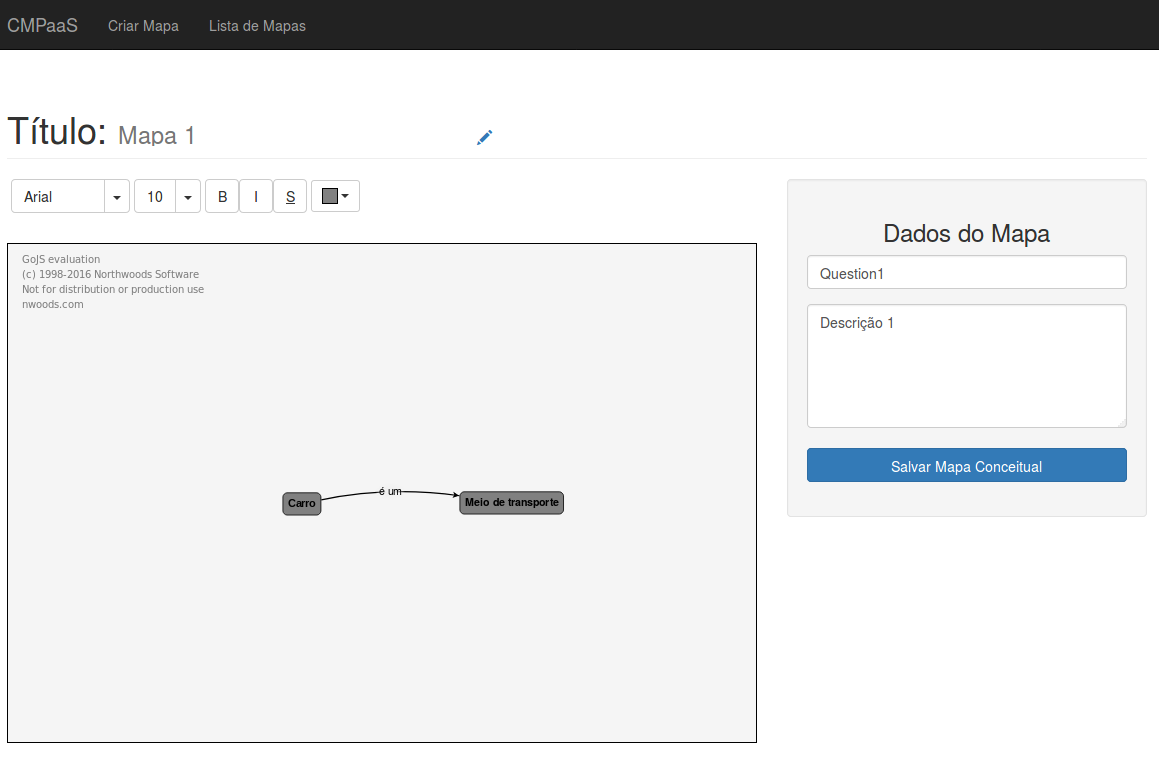
\includegraphics[scale=0.3]{editor.png}
	\end{center}
	\legend{Fonte: Elaborada pelo autor}
\end{figure}

\section{Como usar}

A utilização do plugin é bem simples. Ao acessar uma tarefa o estudante deve clicar no botão de envio de tarefa e ao fazer isto o editor de mapas ira ser mostrado na tela, como na \autoref{fig_editor}. Após criar ou editar o mapa o aluno deve clicar no botão “Salvar alterações” e o json será salvo no banco de dados da plataforma e aparecerá no sumário, conforme \autoref{fig_sumario}. Ao clicar no botão Sincronizar Mapa o diagrama será sincronizado na Nuvem da plataforma CMPaaS.


\begin{figure}[htb]
	\caption{\label{fig_sumario} Sumário da tarefa}
	\begin{center}
		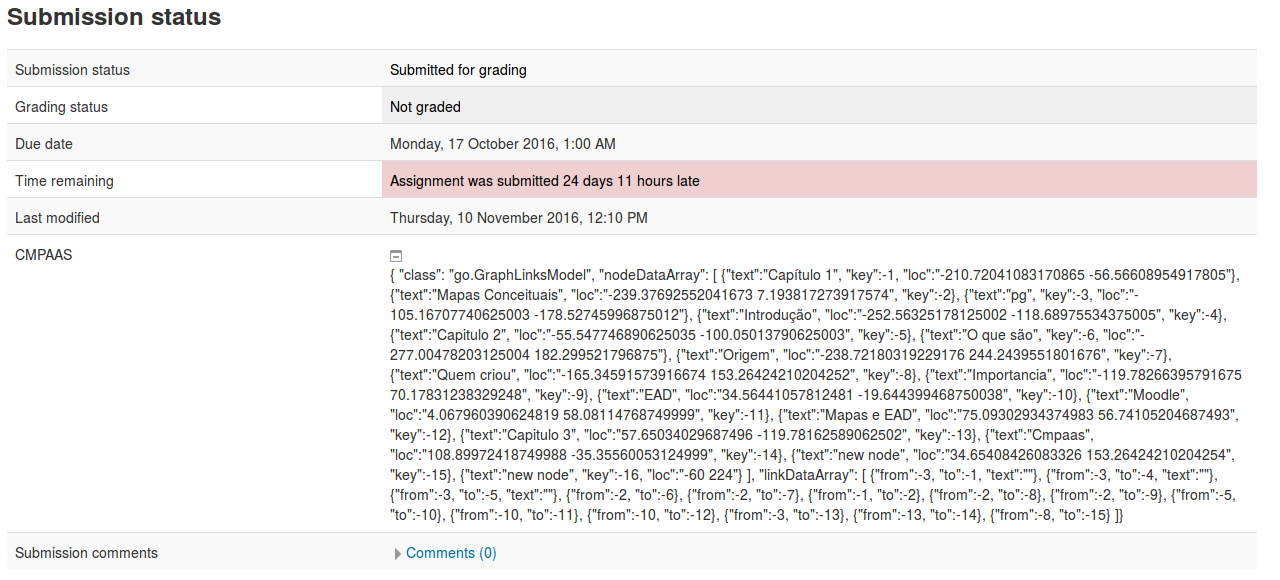
\includegraphics[scale=0.3]{sumario.png}
	\end{center}
	\legend{Fonte: Elaborada pelo autor}
\end{figure}

\section{Provas de Conceitos}

Nesta seção será apresentada a utilização de todas as funcionalidades oferecidas pelo plugin. Elas podem ser dividas em dois grupos, o de recursos para elaboração e edição dos mapas e o de persistência dos diagramas.

Os recursos para edição de mapas são as funções de formatação da aparência do diagrama disponíveis na barra de ferramentas. Elas permitem alterar a cor de preenchimento dos nós e o estilo da fonte de cada conceito. A \autoref{fig_mapa} mostra um mapa no qual foi aplicado estas funções. Já a \autoref{fig_toolbar} apresenta o conteúdo dos menus dropdown de fonte e cor de preenchimento do nó.

Já a persistência do diagrama pode ser divida em duas, a gravação do mapa no Moodle e a sincronização com o CMPaaS. A primeira ocorre quando o usuário clica no botão Salvar Alterações, que foi apresentado na \autoref{fig_editor}. Já a sincronia com o CMPaaS ocorre quando o estudante utiliza o botão Sincronizar Mapa, que pode ser visto na cor verde na \autoref{fig_mapa}.

\begin{figure}[htb]
	\caption{\label{fig_mapa} Mapa que utiliza os recursos de formação}
	\begin{center}
		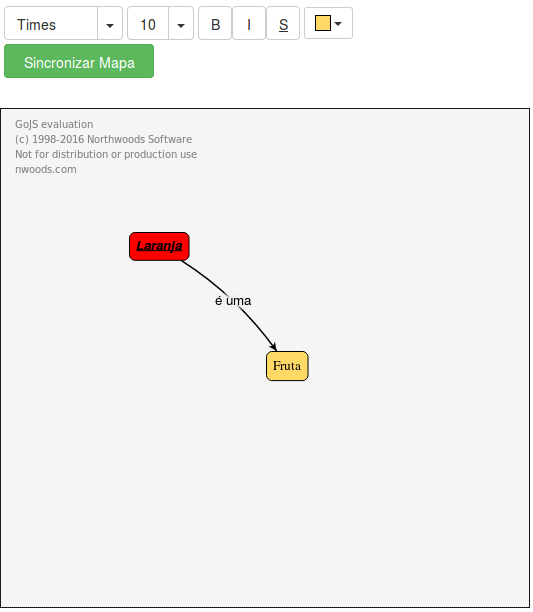
\includegraphics[scale=0.3]{mapa.png}
	\end{center}
	\legend{Fonte: Elaborada pelo autor}
\end{figure}

\begin{figure}[htb]
	\caption{\label{fig_toolbar} Menus dropdown da barra de ferramentas}
	\begin{center}
		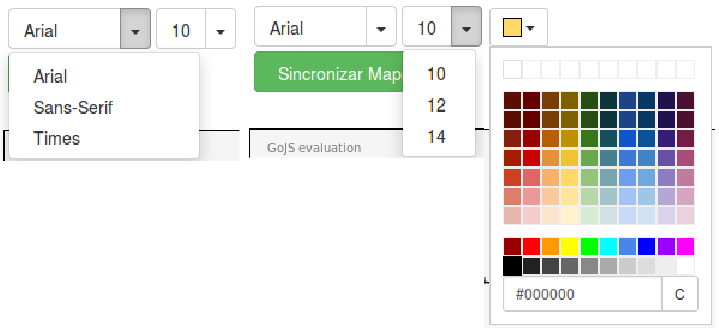
\includegraphics[scale=0.3]{toolbar.png}
	\end{center}
	\legend{Fonte: Elaborada pelo autor}
\end{figure}

% ----------------------------------------------------------
% Finaliza a parte no bookmark do PDF
% para que se inicie o bookmark na raiz
% e adiciona espaço de parte no Sumário
% ----------------------------------------------------------
\phantompart

% ---
% Conclusão
% ---
\chapter{Considerações finais}

\section{Resultados}

O objetivo deste trabalho foi a criação de uma ferramenta que permitisse a utilização de mapas conceituais em cursos gerenciados pela plataforma Moodle. Para realizar isto foi idealizado o desenvolvimento de um módulo de envio de tarefa que oferecesse a possibilidade do estudante responder uma atividade com a elaboração de um mapa conceitual. A ferramenta deveria prover também uma interface para um professor ou tutor visualizar o mapa criado pelo estudante e avaliar o mesmo. Adicionalmente o módulo ofereceria uma interface de integração com o plataforma CMPaaS.

O protótipo desenvolvido neste trabalho alcançou o objetivo de oferecer uma ferramenta para o estudante reponder uma tarefa com mapas  conceituais. O módulo desenvolvido possui um editor de mapas que permite a elaboração de diagramas e modificação de sua aparencia, além de realizar a persistencia dos mapas criados. 

A integração com o CMPaaS também foi implementada, assim o estudante tem a possibilidade de sincronizar o mapa criado no editor com o serviço de armazenamento na Nuvem oferecido pela plataforma. Já a interface para que o mapa seja visualizado para avaliação não foi implementada no protótipo, porém o módulo desenvolvido permite que este recurso seja adicionado em trabalhos futuros.  



\section{Conclusão}

Neste trabalho foi apresentada a definição de mapas conceituais e a sua importância para a educação. Neste contexto foi discutido como eles podem ser utilizados no ensino e foi levantado quais são as ferramentas disponíveis para criação e manipulação de mapas. Neste levantamento foi identificada uma carência de aplicações computacionais que proporcionam suporte a criação de mapas conceituais e a necessidade do desenvolvimento de novas ferramentas com esta finalidade.

Foi pensado então no projeto de uma ferramenta que proporcionasse a aplicação de mapas conceituais na Educação a Distância. Escolhemos o Moodle como a plataforma onde seria realizada a implementação deste projeto. Ele foi escolhido por ser um gerenciador de cursos open-source amplamente utilizado em todo o mundo e por ser facilmente estensível através de inclusão de novos módulos.

Um plugin que permite a aplicação de mapas conceituais em tarefas dos cursos do Moodle foi então desenvolvido. Este plugin possibilida que os estudantes respondam tarefas com a elaboração de mapas conceituais e oferece a possibilidade de sincronização do mapa na plataforma CMPaaS. 

O módulo que foi criado neste trabalho trata-se de um protótipo, sendo assim, não está totalmente funcional e carece de melhorias. No entanto serve como base para a criação de uma ferramenta que pode ser adicionada a lista de repositórios de plugin do Moodle, ampliando assim a possibilidade do uso de mapas conceituais no ensino.         

\section{Trabalhos futuros}
% ---

O protótipo desenvolvido neste trabalho teve foco na interface para o estudante criar mapas conceituais, não possuindo o recurso de apresentar o mapa elaborado nele para um avaliador. Assim a criação de uma forma visualizar o mapa submetido pelo estudante é uma proposta de trabalho futuro. 

Ademais é sugerido o desenvolvimento de trabalhos que visam a melhoria da experiência do usuário que utiliza o editor de mapas. Visto que este trabalho não teve como foco a criação de uma interface otimizada.

% ----------------------------------------------------------
% ELEMENTOS PÓS-TEXTUAIS
% ----------------------------------------------------------
\postextual
% ----------------------------------------------------------

% ----------------------------------------------------------
% Referências bibliográficas
% ----------------------------------------------------------
\bibliography{abntex2-modelo-references}

% ----------------------------------------------------------
% Glossário
% ----------------------------------------------------------
%
% Consulte o manual da classe abntex2 para orientações sobre o glossário.
%
%\glossary

% ----------------------------------------------------------
% Apêndices
% ----------------------------------------------------------

% ---
% Inicia os apêndices
% ---
%\begin{apendicesenv}

% Imprime uma página indicando o início dos apêndices
%\partapendices


%\end{apendicesenv}
% ---


% ----------------------------------------------------------
% Anexos
% ----------------------------------------------------------

% ---
% Inicia os anexos
% ---
%\begin{anexosenv}

% Imprime uma página indicando o início dos anexos
%\partanexos


%\end{anexosenv}

%---------------------------------------------------------------------
% INDICE REMISSIVO
%---------------------------------------------------------------------
%\phantompart
%\printindex
%---------------------------------------------------------------------

\end{document}
